\chapter{T-06: Robustez adversarial y equidad}

\section{Batería adversarial v1}

Se evaluó el checkpoint oficial sobre \texttt{test\_adversarial.csv} ($n=75$, familias A--E). Esta métrica es \textbf{diagnóstica} y no sustituye el F1 oficial del test principal.

\begin{itemize}[noitemsep]
  \item Manifiesto: \texttt{adversarial\_battery\_manifest.json} (SHA-256 versionado).
  \item Resultado global: 45/75 aciertos (60\%).
  \item F1-macro diagnóstico: 0.5314.
  \item FN en amenazas: 10 de 16 casos de amenaza/violencia.
\end{itemize}

\section{Resultados por familia}

\begin{table}[H]
  \centering
  \caption{Batería adversarial por familia (mBERT oficial)}
  \label{tab:adversarial-families}
  \begin{tabular}{llccc}
\toprule
Fam. & Grupo & Resultado & Conf. & n \\
\midrule
A & A. Ofuscación de groserías & 18/20 & 0.9190 & 20 \\
B & B. Emojis & 7/18 & 0.9115 & 18 \\
C & C. Amenazas ofuscadas & 6/11 & 0.9683 & 11 \\
D & D. Jerga salvadoreña inofensiva & FPR 12/14 & 0.8983 & 14 \\
E & E. Control sin jerga & FPR 0/12 & 0.9650 & 12 \\
\bottomrule
\end{tabular}

\end{table}

\begin{figure}[H]
  \centering
  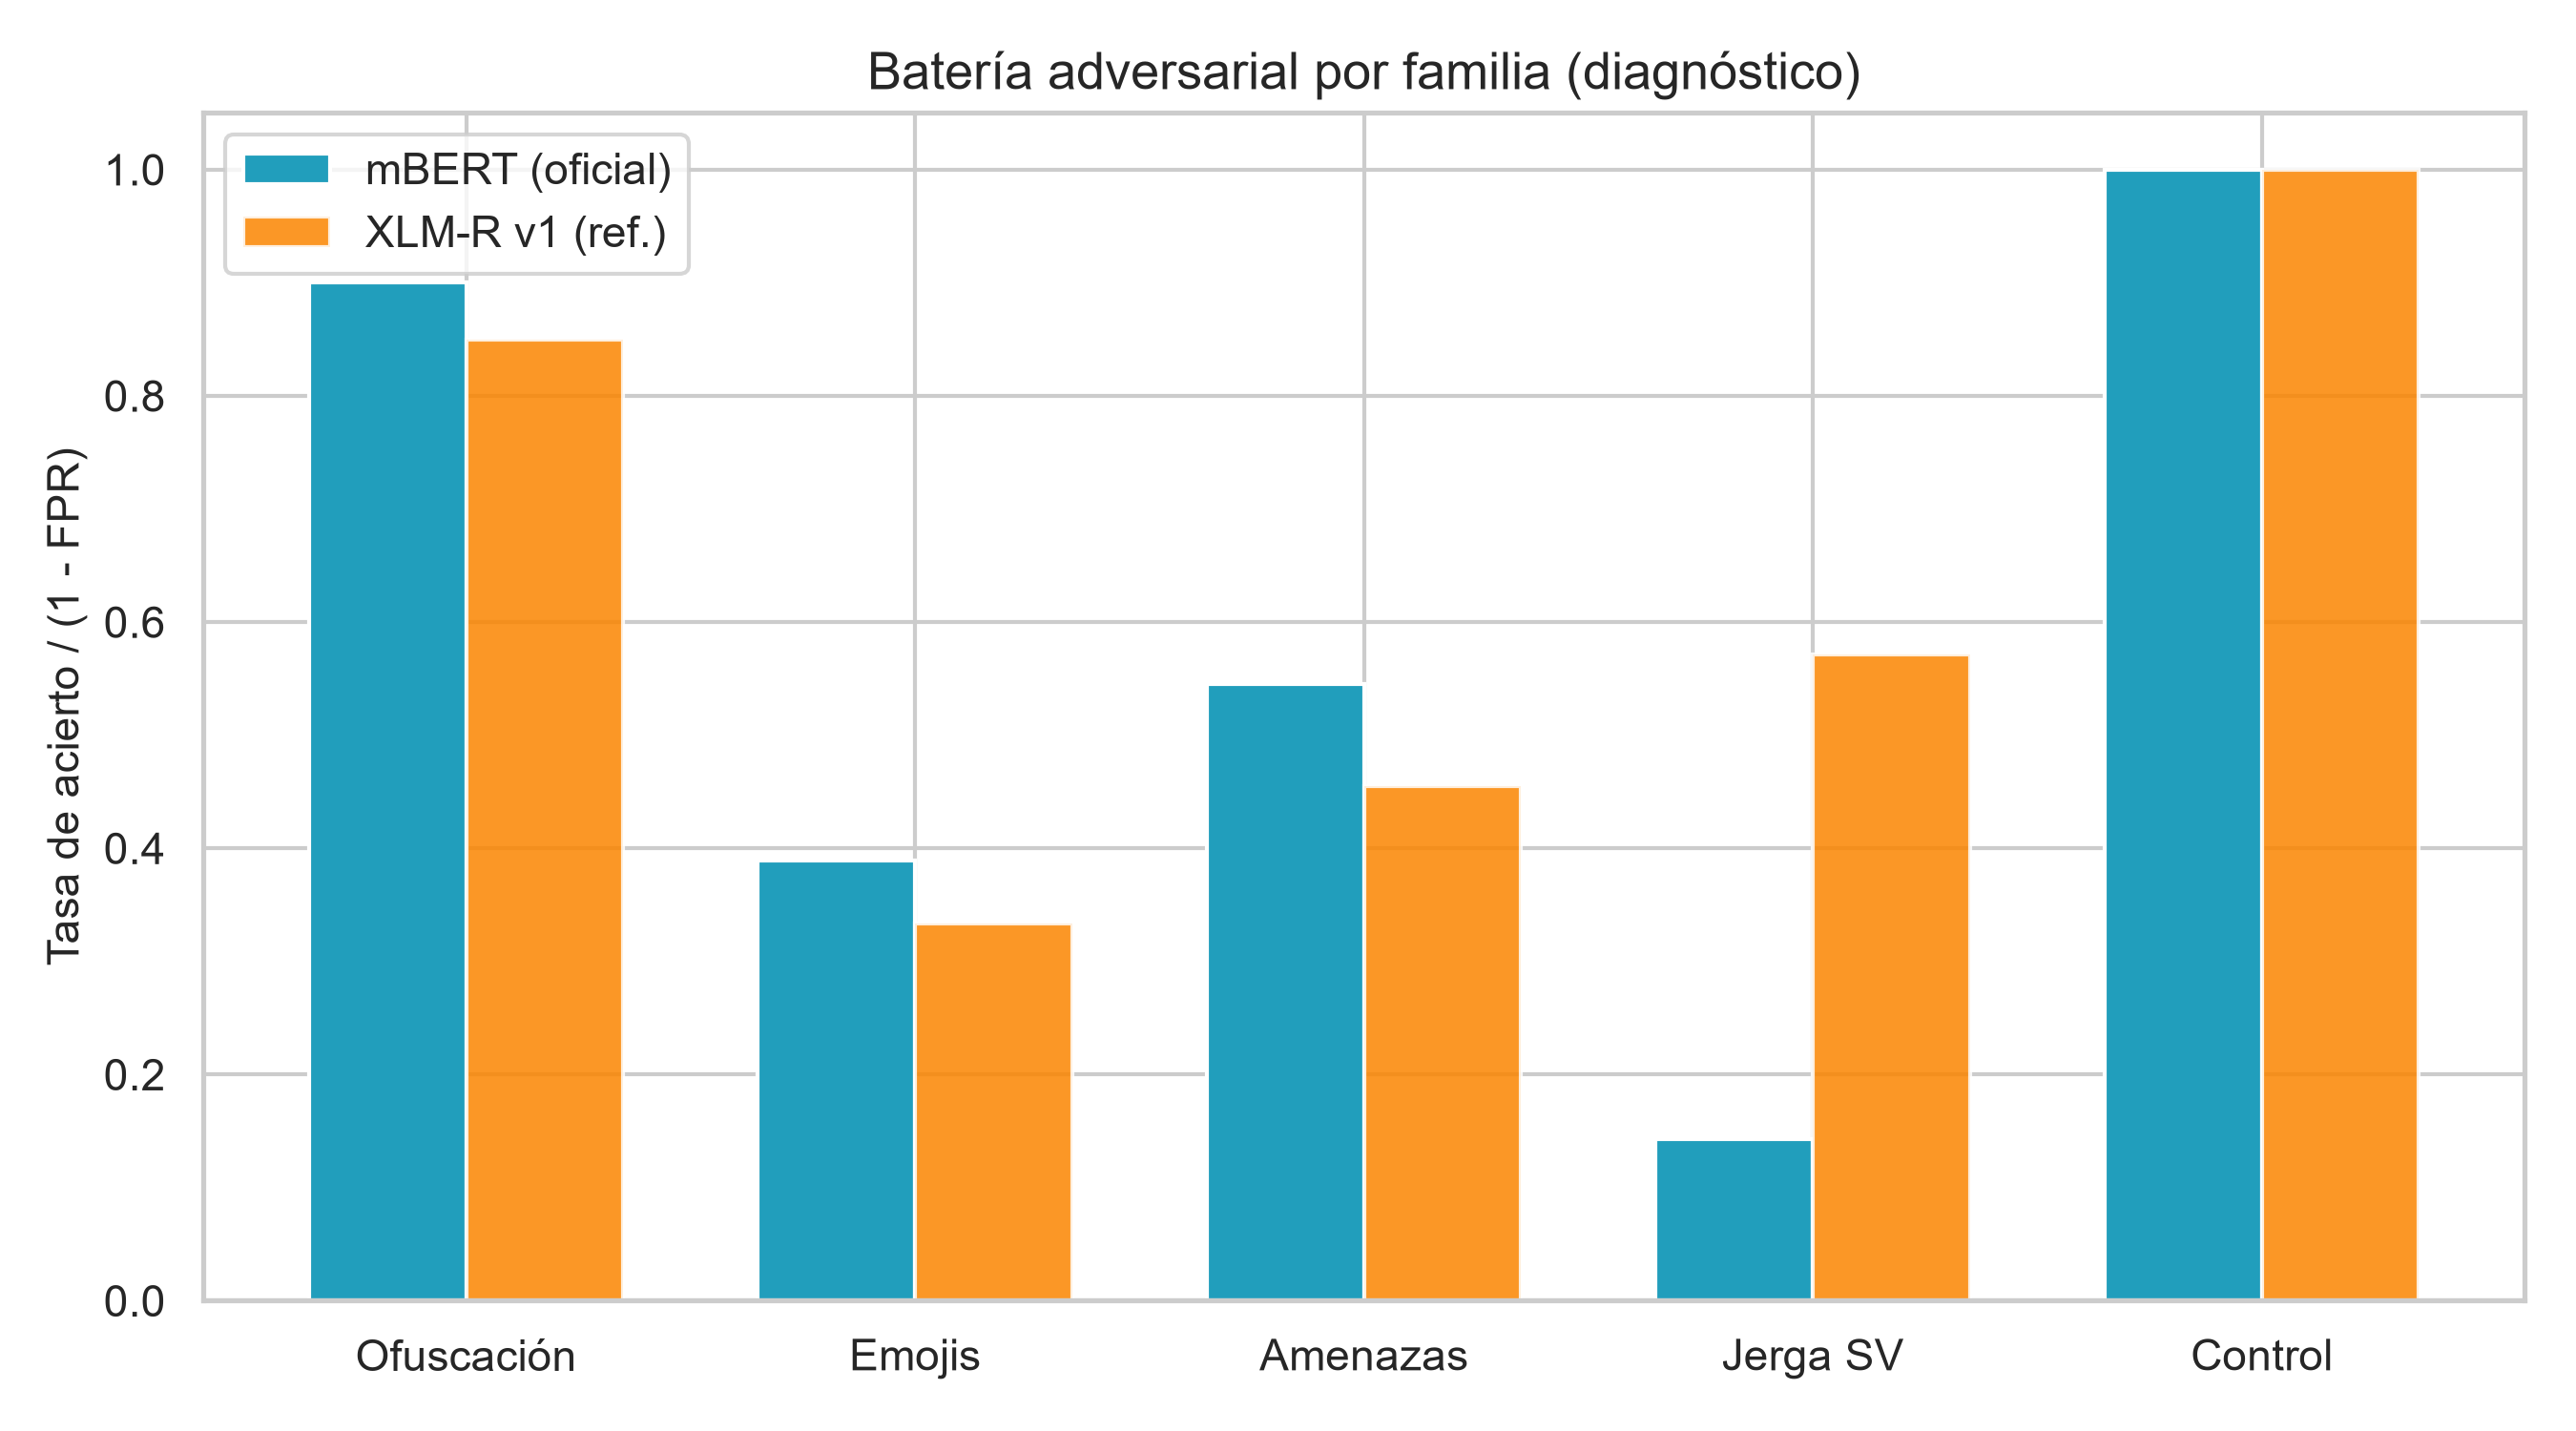
\includegraphics[width=0.85\textwidth]{11_adversarial_families.png}
  \caption{Comparación por familia (mBERT vs referencia XLM-R v1)}
  \label{fig:adversarial}
\end{figure}

\section{Equidad dialectal (familias D vs E)}

\begin{table}[H]
  \centering
  \caption{FPR dialectal en batería adversarial}
  \label{tab:adversarial-dialect}
  \begin{tabular}{lccccr}
\toprule
Grupo & FP/n & FPR & IC lo & IC hi & n \\
\midrule
Jerga SV & 12/14 & 0.8571 & 0.6006 & 0.9599 & 14 \\
Español estándar & 0/12 & 0.0000 & 0.0000 & 0.2425 & 12 \\
\bottomrule
\end{tabular}

\end{table}

El FPR en jerga inofensiva (familia D) es 12/14 (85.7\%) frente a 0/12 en control (familia E). Los intervalos Wilson no se solapan ($\Delta \approx 0.857$).

\section{Intento de mitigación B2}

Se reentrenó un candidato (\texttt{models/mbert-sv-b2}) excluyendo solapamiento con la batería. Mejora adversarial (59/75) pero \textbf{degrada} el test oficial:

\begin{table}[H]
  \centering
  \caption{Antes/después de mitigación B2}
  \label{tab:adversarial-before-after}
  \begin{tabular}{llccccr}
\toprule
Etapa & Checkpoint & F1 test & C & B & FPR gap & Adv. \\
\midrule
baseline & checkpoint-1072 & 0.7777 & 6/11 & 7/18 & 0.8571 & 45/75 \\
candidate\_b2 & checkpoint-1072 & 0.7161 & 11/11 & 15/18 & 0.2857 & 59/75 \\
\bottomrule
\end{tabular}

\end{table}

\textbf{Decisión:} no adoptar B2. Se mantiene \texttt{checkpoint-1072} como modelo oficial (F1 0.7777).

\section{Scripts y tests}

\begin{itemize}[noitemsep]
  \item \texttt{scripts/evaluate\_adversarial.py}, \texttt{scripts/run\_t06\_pipeline.py}
  \item \texttt{src/discurso\_odio/evaluation/adversarial.py}
  \item \texttt{tests/test\_adversarial\_eval.py}
\end{itemize}

\textbf{Criterio de cierre:} brechas documentadas, mitigación evaluada con tradeoffs explícitos, batería versionada sin fuga a val/test.
